\begin{homeworkProblem}

\textbf{Running Time of Value Iteration}

In this problem we construct an example to bound the number of steps it will take to find the optimal policy using value iteration. Consider the infinite MDP with discount factor $\gamma<1$ illustrated in Figure \ref{fig:value_iteration}. It consists of 3 states, and rewards are given upon taking an action from the state. From state $s_0$, action $a_1$ has zero immediate reward and causes a deterministic transition to state $s_1$ where there is reward +1 for every time step afterwards (regardless of action). From state $s_0$, action $a_2$ causes a deterministic transition to state $s_2$ with immediate reward of $\frac{\gamma^2}{1-\gamma}$ but state $s_2$ has zero reward for every time step afterwards (regardless of action).
\begin{figure}[h]
    \centering
    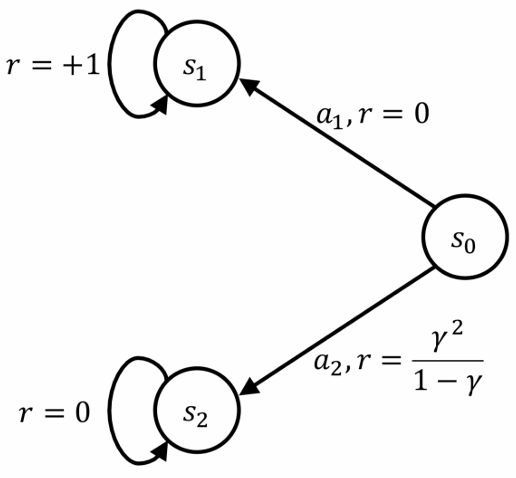
\includegraphics[width=0.4\textwidth]{./figure/value_iteration.png}
    \caption{infinite 3-state MDP}
    \label{fig:value_iteration}
\end{figure}

(a) What is the total discounted return $\left(\sum\limits_{t=0}^{\infty} \gamma^t r_t\right)$ of taking action $a_1$ from state $s_0$ at time step $t=0$?

(b) What is the total discounted return $\left(\sum\limits_{t=0}^{\infty} \gamma^t r_t\right)$ of taking action $a_2$ from state $s_0$ at time step $t=0$? What is the optimal action?

(c) Assume we initialize value of each state to zero, (i.e. at iteration $n=0, \forall s$ : $V_{n=0}(s)=0$). Show that value iteration continues to choose the sub-optimal action until iteration $n^*$ where,
$$n^* \geq \frac{\log (1-\gamma)}{\log \gamma} \geq \frac{1}{2} \log \left(\frac{1}{1-\gamma}\right) \frac{1}{1-\gamma}$$
Thus, value iteration has a running time that grows faster than $\frac{1}{1-\gamma}$. (You just need to show the first inequality)

\solution

(a) The total discounted return of taking action $a_1$ is:
$$\sum_{t=0}^{\infty} r_t \gamma^t = 0 + \sum_{t=1}^{\infty} \gamma^t = \dfrac{\gamma}{1-\gamma}$$

(b) The total discounted return of taking action $a_2$ is:
$$\sum_{t=0}^{\infty} r_t \gamma^t = \frac{\gamma^2}{1-\gamma} + 0 = \dfrac{\gamma^2}{1-\gamma}$$
Since $\gamma < 1$, so it must have $\dfrac{\gamma}{1-\gamma}>\dfrac{\gamma^2}{1-\gamma}$ i.e. the optimal action is $a_1$.

(c) Since state $s_1$ and $s_2$ are the absorbing states, thus directly apply Bellman Expectation Equation, we can get that
\begin{align*}
V_{n+1}(s_1) &= 1 + \gamma V_n(s_1) \Rightarrow V_n(s_1)=\dfrac{1-\gamma^n}{1-\gamma} \\
V_{n+1}(s_2) &= \gamma V_n(s_2) = 0
\end{align*}
As for state $s_0$, we need to consider its actions, thus we need the state-action values:
\begin{align*}
Q_{n+1}(s_0, a_1) &= 0 + \gamma V_n(s_1) = \gamma \dfrac{1-\gamma^n}{1-\gamma} \\
Q_{n+1}(s_0, a_2) &= \dfrac{\gamma^2}{1-\gamma} + \gamma V_n(s_2) = \dfrac{\gamma^2}{1-\gamma} \\
\end{align*}
Thus when $Q_{n+1}(s_0, a_1)\geq Q_{n+1}(s_0, a_2)$, we will selection action $a_1$. Thus $n*$ is the minimal iteration number such that $Q_{n+1}(s_0, a_1)\geq Q_{n+1}(s_0, a_2)$. Thus we can get $n*$ by solving
$$\gamma \dfrac{1-\gamma^n}{1-\gamma} \leq \dfrac{\gamma^2}{1-\gamma}$$
Solve the inequality, we have
$$n^* \geq \dfrac{\log(1-\gamma)}{\log \gamma}$$
So above all, we have proved that the value iteration continues to choose the sub-optimal action until iteration $n^*$  where
$$n^* \geq \dfrac{\log(1-\gamma)}{\log \gamma}$$

For the second inequality, which is easy to prove. The base for the log function should be $2$. Since $0<\gamma<1$, thus what we need to prove is that
\begin{align*}
\frac{\log (1-\gamma)}{\log \gamma} &\geq \frac{1}{2} \log \left(\frac{1}{1-\gamma}\right) \frac{1}{1-\gamma} \\
\Rightarrow \log\gamma + 2(1-\gamma) &\leq 0
\end{align*}
Let $f(\gamma)=\log\gamma + 2(1-\gamma)\Rightarrow f'(\gamma)=\log\gamma+2(1-\gamma), f''(\gamma)=-\frac{1}{\gamma^2}<0$, thus
$$f(\gamma)\leq f\left(\frac{1}{2}\right)=1 - \log 2 = 0\qquad\text{If base is $2$}$$
So above all, we have proved that
$$n^* \geq \frac{\log (1-\gamma)}{\log \gamma} \geq \frac{1}{2} \log \left(\frac{1}{1-\gamma}\right) \frac{1}{1-\gamma}$$

\end{homeworkProblem}

\newpage